\chapter{Cifras de Bloco}
\label{cha:cifras-de-bloco}

No capítulo anterior mostramos que somos capazes de construir um sistema seguro contra ataques do tipo {\em ciphertext only}.
Para isso precisamos supor a existência um gerador de números pseudo-aleatórios, ou seja, um algoritmo capaz de gerar uma sequência de bits indintinguível, para todos efeitos práticos, de uma sequência aleatória.
Nossa definição de ataque é um pouco mais fraca do que a apresentada no Capítulo \ref{cha:sigilo-perfeito}, mas nosso sistema não requer chaves tão grandes.
As cifras de fluxo, porém, compartilham com o OTP dois problemas: são totalmente inseguras caso haja repetição de chaves e não apresentam qualquer garantia de segurança caso o adversário conheça partes do mensagem.

O modelo das cifras de fluxo é adequado para descrever as Máquinas Enigma utilizadas pelo exército nazista nos anos 40.
Sua cifra, porém, foi derrotada não apenas pelo desenvolvimento tecnológico que levou a contrução da máquina Bombe e do Colossus, mas porque os aliados tiveram acesso a trechos de mensagens descriptografas.
Com a teoria da criptografia moderna, diríamos hoje que o tipo de ataque que os ingleses fizeram foi do tipo {\em known plaintext}.

Neste capítulo nos voltaremos para um modelo de ataque ainda mais poderoso.
Ataques do tipo {\em chosen plaintext} (CPA) supõe que o adversário, além de acessar o texto cifrado, é capaz de fazer com que o sistema produza as cifras de mensagens produzidas por ele \cite{Bellare97}.
É evidente que um ataques do tipo {\em known plaintext} são casos particulares deste, mas existem situações em que devemos assumir esse poder maior por parte do adversário.

Vamos formalizar segurança contra ataques CPA de forma análoga à segurança contra ataques {\em ciphertext only}.
O modelo de ameaças é formalizado por meio do seguinte jogo:
\begin{enumerate}
\item O adversário $\mathcal{A}$ escolhe duas mensagens $m_0$ e $m_1$ com o mesmo tamanho ($|m_0| = |m_1|$) e envia para o sistema $\Pi$.
\item O sistema gera uma chave $k$ usando o algoritmo $Gen$ e sorteia aleatoriamente uma das mensagens para criptografar ($\Pi$ sorteia $b \leftarrow \{0, 1\}$ e criptografa $m_b$).
\item Durante todo o processo (mesmo depois de receber a cifra) $\mathcal{A}$ pode consultar o sistema $\Pi$ sobre como uma série de mensagens $q_0, \dots, q_{n'-1}$ seriam criptografadas.
\item A cifra produzida $E(k, m_b) = c$ e enviada de volta para o adversário.
\item O adversário $\mathcal{A}$ produz um bit $b' \in \{0,1\}$.
\end{enumerate}

\begin{center}
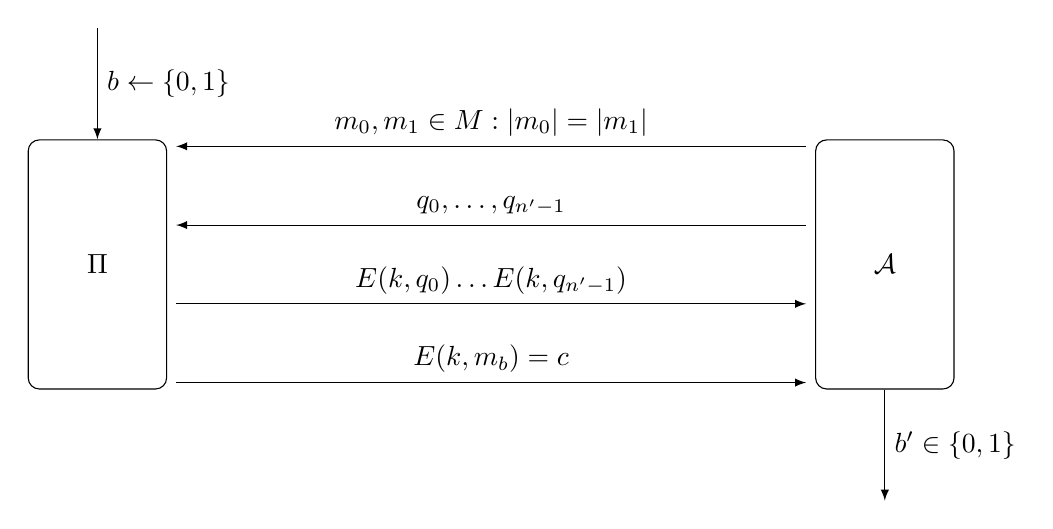
\begin{tikzpicture}[node distance=2cm,auto,>=latex]
\tikzset{
  player/.style={draw,shape=rectangle,rounded corners,minimum width=5em,minimum height=9em}
}
\node[player] (system) {$\Pi$};
\node[player] (adversary) at (10,0) {$\mathcal{A}$};
\draw[->] (9,1.5) -> node[above]{$m_0, m_1 \in M : |m_0| = |m_1|$} (1,1.5);
\draw[->] (9,0.5) -> node[above]{$q_0, \dots, q_{n'-1}$} (1,0.5);
\draw[->] (1,-0.5) -> node[above]{$E(k, q_0) \dots E(k, q_{n'-1})$} (9,-0.5);
\draw[->] (1,-1.5) -> node[above]{$E(k,m_b) = c$} (9,-1.5);
\draw[->] (0,3) -> node{$b \leftarrow \{0,1\}$} (system);
\draw[->] (adversary) -> node{$b' \in \{0,1\}$} (10,-3);
\end{tikzpicture}
\end{center}

A garantia de segurança é idêntica a da cifra de fluxo.
O desafio de $\mathcal{A}$ é acertar qual das duas mensagens foi encriptada.
Chamamos o experimento de $PrivK^{cpa}_{\Pi, \mathcal{A}}$:
\begin{displaymath}
  PrivK^{cpa}_{\Pi, \mathcal{A}}(n) = \left\{
    \begin{array}{lcl}
      1 & \textrm{se} & b = b'\\
      0 & \textrm{c.c.} &\\
    \end{array}
    \right.
\end{displaymath}

Um sistema $\Pi$ é {\em seguro contra CPA} se para todo adversário polinomial $\mathcal{A}$ temos que existe uma função desprezível $\varepsilon$ tal que:
\begin{displaymath}
  Pr[PrivK^{cap}_{\Pi, \mathcal{A}} = 1] \leq \frac{1}{2} + \varepsilon(n)
\end{displaymath}

Para construir um sistema seguro contra CPA assumiremos a existência de {\em funções pseudoaleatórias}.
Considere o conjunto de todas as funções $f: \{0,1\}^n \to \{0,1\}^n$.
Chamaremos esse conjunto de $Func_n$ e não é difícil calcular que $|Func_n| = 2^{n2^n}$.
Gostaríamos de escolher aleatoriamente uma função $f \leftarrow Func_n$, mas isso não é possível, o melhor que podemos fazer é escolher uma chave $k \leftarrow \{0,1\}^n$ e tentar produzir uma função $f_k: \{0,1\}^n \to \{0,1\}^n$ que se pareça com uma função escolhida aleatoriamente.
Assim, como um PRG, uma {\em função pseudoaleatória} (PRF) é tal que não existe algoritmo efeciente capaz de distingui-la de uma função aleatória com probabilidade considerável \cite{Goldreich86}.

Uma {\em cifra de bloco} é uma {\em permutação pseudoaleatória} (PRP), uma função bijetora $p_k: \{0,1\}^n \to \{0,1\}^n$ (permutação), cuja inversa $p_k^{-1}$ pode ser calculado de maneira eficiente e não existe algoritmo polinomial capaz de distinguir $p_k$ de uma permutação aleatória com probabilidade não desprezível.

Uma {\em cifra de bloco} é capaz de criptografar uma mensagem de tamanho fixo $m \in \{0,1\}^n$, chamado de {\em bloco}, $p_k(m) = c$ e decifrar usando sua inversa $p_k^{-1}(p_k(m)) = m$.
Na próxima seção mostraremos como combinar os blocos para criptografar um mensagem de tamanho arbitrário e provaremos a segurança desses sistemas.

\section{Modos de Operação}
\label{sec:modos-de-operacao-bloco}

Uma cifra de bloco é usada para criptografar um bloco de tamanho fixo, por exemplo 128 bits no caso do AES e 64 bits no caso do DES.
Tipicamente, porém, desejamos criptografar uma mensagem de tamanho arbitrário $m \in \{0,1\}^*$.
Para tanto temos que combinar de alguma forma os blocos criptografados pelas cifra de bloco.
A forma mais natural, e insegura, de fazer isso é chamada {\em Eletronic Code Book} (ECB).
Neste {\em modo de operação} dividimos a mensagem $m$ em pedaços do tamanho do bloco ($m = m_0 || m_1 || \dots || m_l$ onde $|m_i| = n$), usamos a cifra de bloco $p_k$ para criptografar cada bloco e contatenos eles, ou seja, $c = p_k(m_0) \dots p_k(m_l)$.
Este modo de operação não garante a segurança contra ataques {\em ciphertext only} porque blocos iguais são criptografados de maneira igual.
Considere o seguinte adversário $\mathcal{A}$ que derrota esta cifra:
\begin{enumerate}
\item $\mathcal{A}$ envia $m_0 = m||m$ e $m_1=m||m'$ para $\Pi$ de forma que $m \neq m'$ e $|m| = |m'| = n$ onde $n$ é o tamanho do bloco,
\item $\Pi$ vai sortear uma das duas mensagens ($b \leftarrow \{0,1\}$) e devolve $E(k, m_b) =c$,
\item se $c$ for formado por dois blocos idênticos $\mathcal{A}$ devolve $0$, caso contrário devolve $1$.
\end{enumerate}

\begin{figure}[!htp]
  \centering
  \includegraphics[width=.5\textwidth]{imagens/ECB.png}
  \caption{Modo ECB}
\end{figure}

\begin{figure}[!htp]
  \centering
  \includegraphics[width=.3\textwidth]{imagens/Tux.jpg}
  \includegraphics[width=.3\textwidth]{imagens/Tux_ecb.jpg}
  \caption{Imagem criptografada no modo ECB}
\end{figure}

Essa maneira ingênua de combinar os blocos não garante a segurança contra o modelos de ataque mais simples que apresentamos.
Queremos um sistema que seja seguro contra CPA.

Pela definição de segurança contra CPA que apresentamos, o adversário possui acesso a um oráculo que ele pode consultar para verificar como uma mensagem seria criptografada.
Essa definição força o algoritmo $E$ de criptografia a ser não determinístico.
Caso contrário, o adversário poderia derrotar o sistema simplesmente enviando duas mensagens que cuja cifra ele consultou.

Para garantir o não determinismo do sistema incluiremos um bloco aleatório no começo da mensagem chamado de {\em vetor inicial}.
Como no caso da cifra de fluxo, o vetor inicial não é um segredo, mas garante que toda mensagem será criptografada de maneira diferente.

No modo de operação {\em Cipher Block Chaining} cada bloco depende não apenas da cifra de bloco $p$ e do bloco $m_i$ a ser encriptado, mas também da cifra do bloco imediatamente anterior $c_{i-1}$.
O algoritmo $E(k,m) := c_0 c_1 \dots c_l$ onde cada $c_i$ tem o tamanho de um bloco $n$ e cada $c_i$ é computado da seguinte maneira:

\begin{eqnarray*}
  c_0 & := & IV \leftarrow \{0,1\}^n \\
  c_i & := & p_k(c_{i-1} \xor m_i) \textrm{ para cada } i = 0, \dots, l
\end{eqnarray*}

Para descriptografar precisamos aplicar $D(k,c) := m_0 \dots m_l$ da seguinte forma:
\begin{eqnarray*}
  m_{i} & := & p_k^{-1}(c_{i+1}) \xor c_{i} \textrm{ para cada } i = 0, \dots, l-1
\end{eqnarray*}

É possível provar que este sistema é seguro contra CPA.

\begin{theorem}
  Se $p$ é uma PRP então o sistema $\Pi$ tal qual apresentado acima, modo CBC, é seguro contra CPA.
\end{theorem}

\begin{figure}[!htp]
  \centering
  \includegraphics[width=.5\textwidth]{imagens/CBC.png}
  \caption{Modo CBC}
\end{figure}


A principal limitação do modo CBC é que os blocos precisam ser processados em sequência, ou seja, o algoritmo não é paralelizável.
O {\em modo contador} (Ctr), por outro lado, não tem essa limitação.
Este modo opera de maneira muito similar a uma cifra de fluxo.
Como no modo CBC o primeiro bloco é uma sequência de bits aleatória ($IV$).
Para ada bloco é calculado somando o índice do bloco com $IV$ e aplicado uma função pseudoaleatória ao resultado.
Calculamos por fim o XOR do valor obtido com o bloco da mensagem:
\begin{eqnarray*}
  c_0 & := & IV \leftarrow \{0,1\}^n \\
  c_i & := & m_i \xor f_k(IV + i) \textrm{ para cada } i = 1, \dots, l
\end{eqnarray*} 

O algoritmo $D(k,c)$ é exatamente a mesma coisa, como se poderia esperar:
\begin{eqnarray*}
  m_i & := & c_{i+1} \xor f_k(c_0 + i) \textrm{ para cada } i = 0, \dots, l-1
\end{eqnarray*} 

\begin{figure}[!htp]
  \centering
  \includegraphics[width=.5\textwidth]{imagens/Ctr.png}
  \caption{Modo Contador}
\end{figure}

A segurança do modo contador exige apenas uma função pseudoaleatória que não precisa ser inversível:


\begin{theorem}
  Seja $f$ uma função pseudoaleatória, o sistema $\Pi$ tal qual apresentado acima, modo Ctr, é segura contra CPA.
\end{theorem}
\begin{proof}
  Seja $\Pi$ o sistema de criptografia usando uma função pseudoaleatória em modo Ctr e $\Pi'$ o mesmo sistema, mas usando uma função realmente aleatória.
Usamos o adversário $\mathcal{A}$ para construir um distinguidor $D$ que recebe uma entrada $1^n$ e acesso a um oráculo $O:\{0,1\}^n \to \{0,1\}^n$ da seguinte forma:
\begin{enumerate}
\item Sempre que $\mathcal{A}$ fizer uma consulta a seu oráculo em um mensagem $m$, fazemos o seguinte:
\begin{enumerate}
\item Geramos $IV \leftarrow \{0,1\}^n$.
\item Consultamos $O(IV + i)$ para cada $i \in 0, \dots, l$ para receber $y_0, \dots, y_l$ como resposta.
\item Devolvemos $y_0 \xor m_0 \dots y_l \xor m_l$ para $\mathcal{A}$
\end{enumerate}
\item Quando $\mathcal{A}$ envia $m_0$ e $m_1$ para o sistema, escolhemos $b \leftarrow \{0,1\}$ e:
\begin{enumerate}
\item Geramos $IV \leftarrow \{0,1\}^n$.
\item Consultamos $O(IV + i)$ para cada $i \in 0, \dots, l$ para receber $y_0, \dots, y_l$ como resposta.
\item Devolvemos $y_0 \xor m_{b0} \dots y_l \xor m_{bl}$ para $\mathcal{A}$
\end{enumerate}
\item Quando $\mathcal{A}$ devolve o bit $b'$ devolvemos $1$ se $b = b'$ e $0$ caso contrário.
\end{enumerate}

$D$ opera em tempo polinomial, pois $\mathcal{A}$ também opera em tempo polinomial e conforme ambos operam da maneira idêntica, temos que:

\begin{eqnarray*}
  Pr_{k \leftarrow \{0,1\}^n}[D^{f_k}(1^n) = 1] & = & Pr[PrivK^{cpa}_{\mathcal{A},\Pi}(n) = 1]\\
  Pr_{f \leftarrow Func_n}[D^{f}(1^n) = 1] & = & Pr[PrivK^{cpa}_{\mathcal{A},\Pi'}(n) = 1]
\end{eqnarray*}
 
Como $f$ é uma função pseudoaleatória, por definição, temos que existe $\varepsilon$ desprezível tal que:
\begin{displaymath}
  |Pr_{k \leftarrow \{0,1\}^n}[D^{f_k}(1^n) = 1] - Pr_{f \leftarrow Func_n}[D^{f}(1^n) = 1]| \leq \varepsilon(n)
\end{displaymath}

Juntando tudo temos que:

\begin{displaymath}
  |Pr[PrivK^{cpa}_{\mathcal{A},\Pi}(n) = 1] - Pr[PrivK^{cpa}_{\mathcal{A},\Pi'}(n) = 1]| \leq \varepsilon(n)
\end{displaymath}

Se conseguirmos mostrar que $Pr[PrivK^{cpa}_{\mathcal{A},\Pi'}(n) = 1] < \frac{1}{2} + \varepsilon'(n)$ para um $\varepsilon'$ desprezível, então resolvemos o problema, pois teremos:
\begin{displaymath}
  Pr[PrivK^{cpa}_{\mathcal{A},\Pi}(n) = 1] < \frac{1}{2} + \varepsilon(n) + \varepsilon'(n)
\end{displaymath}

Vamos chamar de $IV$ o primeiro bloco da cifra $c$ produzida pelo sistema $\Pi'$ e $IV_i$ o primeiro bloco de cada cifra $c_i$ resultado das consultas de $\mathcal{A}$ ao oráculo.
\begin{enumerate}
\item Se para nenhuma $IV + j$ usado para encriptar algum bloco $j$ de $m_b$ coincidir com nenhum $IV_i + j'$ de algum bloco $j'$ de uma consulta então $\Pi'$ se comporta exatamente como um OTP e temos que $Pr[PrivK^{cpa}_{\mathcal{A},\Pi'}(n) = 1] = \frac{1}{2}$.
\item Caso contrário é possível que o $\mathcal{A}$ seja capaz de distinguir as mensagens.
\end{enumerate}

Resta, portanto, calcular a probabilidade de uma coincidência como essa ocorrer.
Como $\mathcal{A}$ tem que ser polinomial, o número de consultas máximo que ele pode fazer está limitado a $q(n)$ onde $q$ é um polinômio.
Seja $l$ o número de blocos de $c$ e $l_i'$ o número de blocos da $i$-ésima consulta.
Essa coincidência quando $IV + 1 \dots IV + l$ intersecciona $IV_i + 1 \dots IV_i + l'$, ou seja, quando:
\begin{displaymath}
  IV - l' + 1 \leq IV_i \leq IV + l -1
\end{displaymath}

Ou seja, existem $l + l' - 1$ casos em que ocorre uma intersecção, num universo de $2^n$ valores.
Assim, a probabilidade dessa coincidência é $\frac{l + l' -1}{2^n}$.
Essa probabilidade é maximizada para os maiores valores possíveis de $l$ e $l'$, a saber, $q(n)$.
Portanto a maior probabilidade possível para essa intersecção é $\frac{2q(n) - 1}{2^n}$ que é desprezível.
Concluímos que:

\begin{displaymath}
Pr[PrivK^{cpa}_{\mathcal{A},\Pi'}(n) = 1] < \frac{1}{2} + \frac{2q(n) - 1}{2^n}
\end{displaymath}
\end{proof}

A demonstração indica que o tamanho dos blocos também influencia em sua segurança.
Isso ocorre, pois quanto menos os blocos maior a chance de gerar vetores inciais idênticos, e portanto, de criptografar duas mensagens distintas com a mesma chave.
Como exemplo, tomando o caso concreto do DES, seu bloco tem tamanho $64$ e,portanto, esperamos uma colisão depois de $2^{32}$ blocos (ver Capítulo \ref{cha:hash}), ou cerca de 4Gb.
No momento em que estas notas são escritas, este valor é alto, mas plausível em muitas aplicações práticas.

\section{Construções Práticas}
\label{sec:construcoes-praticas}
Como explicitamos na seção anterior, um PRP é uma permutação $p: \{0,1\}^n \times \{0,1\}^l \to \{0,1\}^l$ em que $n$ é o tamanho da chave e $l$ o tamanho do bloco.
Assim, dado $k \leftarrow \{0,1\}^n$ construímos $p_k$ que deve ser indistinguível na prática de $p \leftarrow Perm(\{0,1\}^l)$.
Não conhecemos um sistema demonstradamente pseudoaleatório, mas os sistemas que apresentaremos, especialmente o AES, tem sido validado na prática.

Nosso desafio será construir um algoritmo em que a mudança de um único bit, seja na mensagem ou na chave, afeta -- mas não necessarimante altera -- todos os bits da cifra.
Para essa tarefa partiremos do paradigma proposto por Shannon chamado de {\em confusão e difusão} \cite{Shannon49}.

A ideia da {\em confusão} é dividir o bloco em partes menores, digamos de 8 bits cada, e aplicar uma tabela que indique para cada sequência de 8 bits da entrada qual seria a saída.
Apenas a confusão não é suficiente para nosso objetivo, pois a alteração do primeiro bit, por exemplo, afetaria apenas os 8 primeiros bits da cifra.
A {\em difusão} então seria responsável por embaralhar os bits, espalhando a mudança de uma partes nas demais partes.
Nas cifras de bloco fases de confusão e difusão são repetidas um número de vezes.

\subsection{Data Encryption Standard (DES)}
\label{sec:des}

O Data Encryption Standard (DES) foi o padrão para a cifras de bloco do fim dos anos 70 até o fim dos anos 90.
Projetado pela IBM o algoritmos sofreu importantes alterações pela NSA antes de se tornar um padrão internacional.

O DES utiliza uma técnica chamada {\em rede de Feistel} (Figura \ref{fig:feistel}) que utiliza uma serie de funções $f_i:\{0,1\}^{l/2} \to \{0,1\}^{l/2}$ para produzir umafunção eficientemente inversível \cite{Feistel73}.
A entrada $m = \in \{0,1\}^l$ da rede é dividia ao meio $L := m_0 \dots m_{(l/2)-1}$ e $R := m_{l/2} \dots m_l$ e em cada rodada $i$ é produzido $L_iR_i$ da seguinte forma:
\begin{displaymath}
  L_i := R_{i-1} \textrm{ e } R_i := L_{i-1} \xor f_i(R_{i-1})
\end{displaymath}


\begin{figure}[htbp]
  \centering
  \includegraphics[width=.8\textwidth]{imagens/feistel.png}
  \caption{Rede de Feistel}
  \label{fig:feistel}
\end{figure}

Dada a saída $\langle L_i, R_i \rangle$ da $i$-ésima rodada de uma rede de Feistel, podemos recuperar o valor de $\langle L_{i-1}, R_{i-1} \rangle$ primeiro fazendo $R_{i-1} := L_i$ e em seguinda calculando:
\begin{displaymath}
  L_{i-1} := R_i \xor f_i(R_{i-1})
\end{displaymath}

Esse procedimento pode ser repetido para todas as rodadas da rede para inverter a função.

O DES é uma rede de Feistel com 16 rodadas.
Ela recebe uma chave de 64 e prontamente descarta 8, portanto, e criptografa blocos de 64 bits, ou seja, $DES: \{0,1\}^{56} \times \{0,1\}^{64} \to \{0,1\}^{64}$.
A chave de 56 passa por um processo chamado {\em key schedule} que produz 16 subchaves de 48 bits.
As funções em cada rodada do DES são identicas, recebem uma subchave de 48 bits e um bloco de 32 bits (metade do bloco total) e produz um bloco de 32 bits $f: \{0,1\}^{48} \times \{0,1\}^{32} \to \{0,1\}^{32}$.
Resta, portanto, apresentar a função $f$ (Figura \ref{fig:feistel-function}):
\begin{enumerate}
\item o bloco é expandido para uma sequência de 48 bits,
\item aplica-se o XOR do bloco expandido com a subchave,
\item o resultado é dividido em 8 pedaços de 6 bits cada,
\item cada pedaço desses passa por um SBox diferente que substitui os 6 bits por 4 bits (fase de confusão),
\item o resultado é reduzido para uma sequência de 32 bits e, por fim,
\item os bits são misturados (fase de difusão).
\end{enumerate}

\begin{figure}[!htp]
  \centering
  \includegraphics[width=.4\textwidth]{imagens/feistel-function.png}
  \caption{Função de Fiestel do DES}
  \label{fig:feistel-function}
\end{figure}


A adoção do padrão DES foi cheia de controvérsias.
Não foi esclarecido o motivo do descarte do 8 bits da chave.
Uma chave de 56 bits é hoje considerada insegura contra um ataque de força bruta e estava no limite da segurança nos anos 70.
Um artigo de 1993 propõe um projeto de hardware que, em teoria, seria capaz de aplicar um ataque força-bruta em uma chave de 56 bits em um dia e meio \cite{}.
Em 1998 a {\em Eletronic Frontier Foundation} (EFF) construiu uma máquina que foi capaz de quebrar a cifra em 56 horas (cerca de dois dias e meio).
A máquina chamada de {\em Deep Crack} custou pouco menos de 250 mil dólares.
Em 2006 pesquisadores alemães desenvolveram um hardware de baixo custo -- cerca de dez mil dólares -- capaz de efetuar um ataque de força-bruta ao DES em menos de uma semana.
Desconfia-se que nos anos 80 apenas governos de grandes potências mundiais tinham recursos necessários para construir máquinas com tal capacidade.
Hoje em dia o algoritmo DES é considerado totalmente inseguro.

% No livro do Paar tem uma definição formal de ataque força bruta e uma análise da probabilidade de coincidência de chaves

Além do pequeno tamanho da chave, e mais suspeito, os S-Boxes foram alterados pela NSA sem grandes explicações antes do algoritmos ser adotado como padrão.
Anos mais tarde pesquisadores apresentaram uma técnica chamada criptoanálise diferencial.
Diversas cifras se tornaram inseguras com o anúncio desta técnica, mas supreendentemente o DES não.
Desconfia-se que os pesquisadores da NSA conheciam a técnica e alteraram a cifra de forma que ela se torna-se segura contra este tipo de ataque.

\subsection{Advanced Encryption Standard (AES)}
\label{sec:aes}

As desconfianças em torno do DES e o ataque força bruta iminete contra sua chave levaram o orgão estadunidense responsável pela estabelecimento de padrões internacionais (NIST) a propor um concurso acadêmico em 1997 para elaboração de um novo padrão.
Cada concorrente, além de propor o algoritmo tinha a tarefa de encontrar vulnerabilidades nos demais algoritmos propostos.
Cinco finalistas foram considerados adequados e em abril de 2000 o algoritmos {\em Rijndael} foi anunciado como vencedor e passou a ser chamado de AES.

O AES criptografa blocos de 128 bits possui três versões: uma com chaves de 128 bits e 10 rodadas, uma com chaves de 196 bits e 12 rodadas e uma com chaves de 256 bits e 14 rodadas.
Diferente do DES, o AES não usa uma rede de Feistel, mas uma técnica que chama-se {\em rede de substituição e permutação}.

O bloco no AES é dividido em 8 sequência de 16 bits que é tratada com um quadrado de 4 por 4 chamado de {\em estado}.
Em cada rodada o algoritmo repete os seguintes passos (Figura \ref{fig:aes}).

\begin{enumerate}
\item {\em AddRoundKey:} O {\em key schedule} do AES produz uma subchave de 128 bits para cada rodada e aplicamos o XOR dessa subchave com o estado.
\item {\em SubBytes:} Cada byte do estado é substituído por um novo byte definido por um SBox único que é bijetor (fase de confusão).
\item {\em ShiftRow:} Rotacionamos a segunda linha do estado em uma posição, a terceira em duas posições e a quarta e três posições para a direita.
\item {\em MixColumns:} As quatro linhas do estado são interpretados com um vetor que é multiplicado por uma matriz específica e fixa. Essa transformação é de tal forma que garante que cada byte de entrada influencie quatro bytes de saída (fase de difusão). 
\end{enumerate}

\begin{figure}[!htp]
  \centering
  \begin{minipage}{.45\textwidth}
    \centering
    \includegraphics[width=\textwidth]{imagens/AddRoundKey.png}  
  \end{minipage}
 \begin{minipage}{.45\textwidth}
    \centering
    \includegraphics[width=\textwidth]{imagens/SubBytes.png}
  \end{minipage}
  \begin{minipage}{.45\textwidth}
    \centering
    \includegraphics[width=\textwidth]{imagens/ShiftRows.png}  
  \end{minipage}
 \begin{minipage}{.45\textwidth}
    \centering
    \includegraphics[width=\textwidth]{imagens/MixColumns.png}
  \end{minipage}
  \caption{Etapas do AES}
  \label{fig:aes}
\end{figure}

Na última rodada a fase {\em MixColumn} é substituída pela {\em AddRoundKey}.
O AES é construído cuidadosamente de forma ser efecientemente inversível na presença da chave.
Até a escrita destas notas não se conhece um ataque contra o AES mais eficiente do que o ataque força bruta.




\section{Exercícios}
\label{sec:exercicios}

\begin{exercicio}
  Considere a definição de segurança contra CPA em que consideramos qualquer adversário $\mathcal{A}$ -- não apenas os eficientes -- e exigimos que $Pr[PrivK^{cpa}_{\Pi,\mathcal{A}}(n) = 1] = \frac{1}{2}$.
  Mostre que é impossível construir um sistema que satisfaça essa definição de segurança.
\end{exercicio}

\begin{exercicio}
Mostre que a operação $R_i \xor f_i(R_{i-1})$ na rede de Feistel de fato recupera o valor de $L_{i-1}$.
\end{exercicio}

\begin{exercicio}
  Mostre que os modos CBC e Ctr são corretos, ou seja, que em ambos os casos $D(k, E(k,m)) = m$;
\end{exercicio}

\begin{exercicio}
  Suponha que $f$ seja uma função pseudo-aleatória com chave e blocos ambos de 128 bits e considere o seguinte sistema:
  \begin{enumerate}
  \item Seleciona aleatoriamente duas sequência de 128 bits, a chave $k$ e o vetor inicial $IV$
  \item Divide a mensagem $m$ em blocos de 128 bits: $m_0, m_1, \dots, m_{n-1}$ (podemos supor que $|m|$ é múltiplo de 128).
  \item A cifra $c = c_0 || c_1 || \dots || c_{n-1}$ é tal que $c_i = m_i \oplus f_k(IV)$ para $i = 0, ..., n-1$
  \item Para descriptografar fazemos $c_i \oplus f_k(IV)$ para $i = 0, \dots, n-1$.
  \end{enumerate}
  Esse sistema é seguro? Por que?
\end{exercicio}

\begin{exercicio}
Suponha que um bit em uma cifra tenha sido alterado por um erro.
Qual o efeito disso na mensagem descriptografada caso a cifra tenha sido produzida usando o modo Ctr? E no caso de ter sido produzida usando o modo CBC?  
\end{exercicio}



